%!TEX root = ../../main.tex
%chktex-file 18

\section{Reinventing Gillian's Logging Structure}\label{sec:log-structure}

The first step of enriching the debugging process was completely restructuring
logs in Gillian. This began with adding logs to the unification process,
which served as both a good introduction to Gillian's logging mechanisms,
and an indication of where they needed improvement.


\subsection{Gillian's Logging Mechanisms}

In order to log a report to the database, one must first create a
\texttt{Loggable.t} and supply it to the relevant log function (see
\autoref{lst:loggable} for the relevant module). Constructing a
\texttt{Loggable.t} essenitally requires a pretty-pretting function (for logging
to the file), and functions to convert the content type to and from a
\texttt{Yojson.Safe.t}, the itermediate representation of a JSON object provided
by the Yojson library~\cite{yojson} (when logging to the database). For the vast
majority of the project, there was no need to consider manually creating
functions for converting types to JSON (and never a need to write one for the
inverse), due to the very helpful `deriving' syntax provided by the
\texttt{ppx\_deriving} library~\cite{ppx-deriving}, and extended for Yojson by
\texttt{ppx\_deriving\_yojson}~\cite{ppx-deriving-yojson}; simply by suffixing a
type with \texttt{[@@deriving yojson]}, JSON conversion functions are
automatically generated for that type. This automatic function definition can
also be performed for pretty printing (\texttt{[@@deriving show]}) and for
the creation of records (\texttt{[@@deriving make]}).

The power of providing both pretty printing and JSON conversion functions came
to light when logging the symbolic state before unifying an assertion; in the
same call to a logging function, the state can be both logged to the database
in JSON format, and prettily logged to the file. The importance of maintaining
the layout of the log file cannot be overstated, as the original creators of
Gillian continue to depend on it for understanding Gillian's internal processes.
While this isn't important to the end user, keeping consistency here was an
absolute requirement.

A necessary step in preparing to restructure Gillian's logs was to provide more
control over the \texttt{previous} and \texttt{parent} fields of a report.
Internally, Gillian's logging mechanism keeps track of a stack of parent report
IDs (which is used to restore the proper parent ID when `releasing' the current
parent), and the previous report ID (directly used to set the \texttt{previous})
field of a new report. The original logging mechanism only allowed modification
of the parent via the \texttt{with\_phase} function, which `wraps' a thunk with
a \texttt{"phase"} report, i.e.\ setting the parent ID to the newly logged
phase report, executing the thunk, then releasing the phase report parent.
A much finer-grain level of control is required, so a new set of functions
were added to Gillian's \texttt{Logging} module (see
\autoref{lst:logging-parent-previous} and \autoref{lst:reportbuilder}), to allow
manual control over the parent and previous report IDs.


\subsection{Planning a New Log Structure}

Before taking the implementation any further, it was time to take a step back
and plan out the desired logging structure. Care was taken to work with
Gillian's internal processes to provide as much relevant data as possible,
while not rigidly adhering to the internal structure. The new, desired logging
structure (\autoref{fig:log-structure-desired}) more closely resembles the
intuition of symbolic execution and unification, rather than being dictated by
Gillian's internals. There were three driving principles in the formation of this
structure:

\myparagraph{Intiution}:
It's especially important that the logging structure represents the intuitive
process of branched symbolic execution and unification, so that when the
debugger extension is developed, a user-friendly UI can become a natural
consequence of working with the new logging structure. This, naturally, was a
strong influence on the other principles.

\myparagraph{Non-linearity}:
Both symbolic execution and unification can branch; the former when encountering
a branching action such as an if/else statement, and the latter when considering
predicates with multiple cases (as with the \texttt{list} predicate used in this
example). This leverages the fact that in the database, \texttt{previous} is a
many-to-one relation, mirroring how one command can symbolically branch into two
different scenarios.

\myparagraph{Hierarchy}:
The top level of the trace is reserved for the essential outline of the
verification process; each step of symbolic execution, and the unification at
the end of each branch. Any `extra' information, such as the result of executing
a command, unification of a function call, and the assertions performed under a
unification, is reported as the child of the relevant parent report. This
essentially allows any log queries to `step in' to a part of the verification
process by querying the children of a report.

% Temporarily reduce margins to allow the figure to take up more of the page
\newgeometry{top=0.5cm,bottom=2cm,left=1cm,right=1cm}
\begin{sidewaysfigure}
  \center{}
  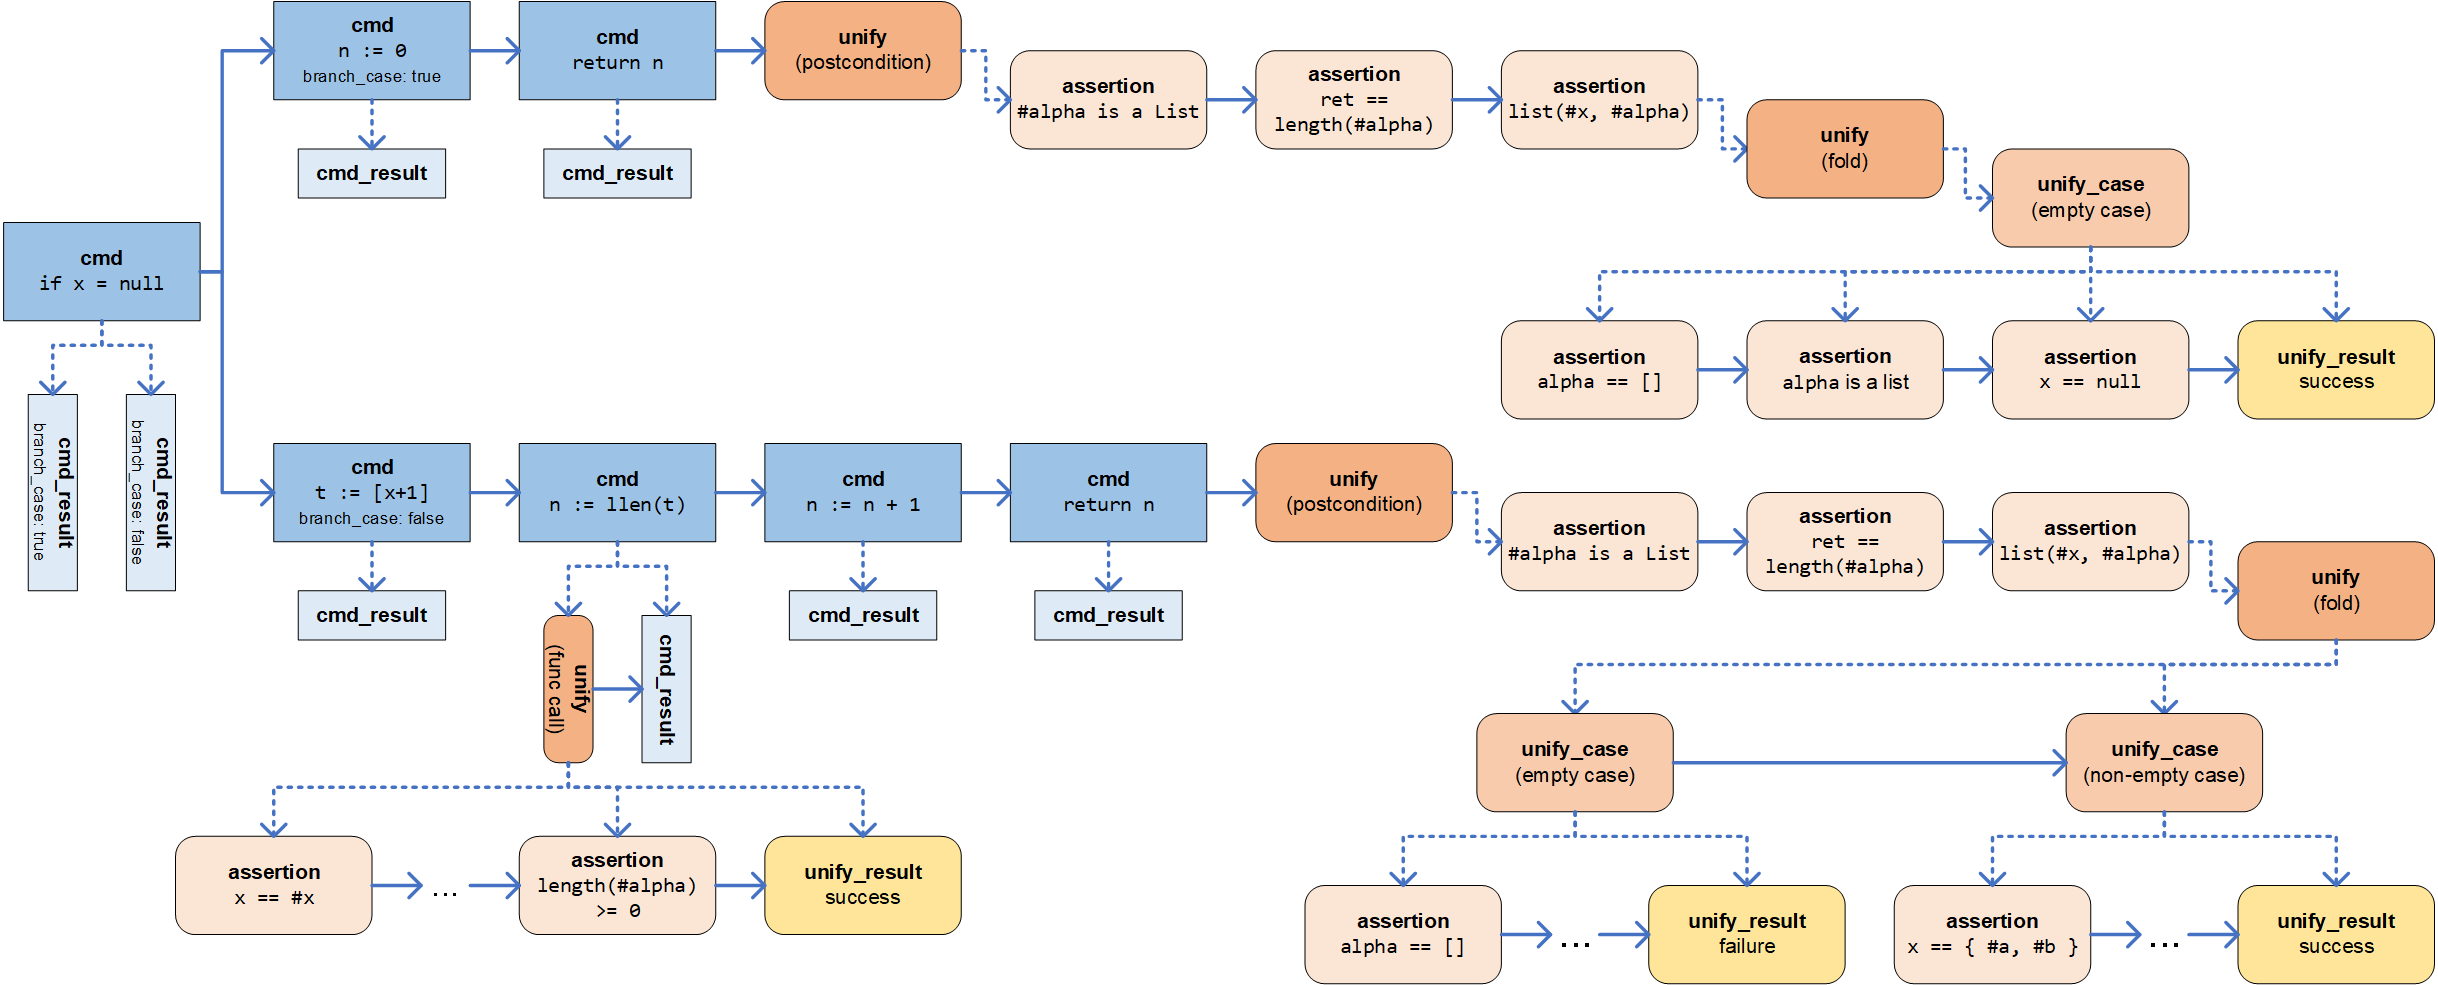
\includegraphics[width=0.95\textwidth]{img/log-structure-desired.png}
  \caption{The new, desired reporting structure}%
  \label{fig:log-structure-desired}
\end{sidewaysfigure}
\restoregeometry{}


\subsection{Implementing the New Log Structure}

The implementation of the ideal log structure began with adding reports for
all the necessary new report types:
\begin{itemize}
  \item \texttt{"cmd"} --- representing the symbolic state \textit{before} a
        step executes a command.
  \item \texttt{"cmd\_result"} --- representing the symbolic state
        \textit{after} executing a command; this replaces \texttt{"cmd\_step"}
        reports in almost all cases.
  \item \texttt{"proc\_init"} --- a replacement for the \texttt{"cmd\_step"}
        report at the very start of symbolic execution; this is a compromise
        in order to preserve the original file log layout, and will be ignored
        during debugging.
  \item \texttt{"unify"} --- denotes the start of unification; includes the
        full unification plan and the symbolic state that will be unified
        against it, as well as the nature of unification (postcondition,
        function call, fold, etc.)
  \item \texttt{"unify\_case"} --- specifies a particular case of unification;
        this comes into play when folding a predicate with multiple cases.
  \item \texttt{"unify\_result"} --- simply denotes the end of unification,
        while specifying whether the unification was a success or failure.
  \item \texttt{"assertion"} --- contains all relevant information about the
        symbolic state being unified against an assertion; this serves as a
        single step in the unification process.
\end{itemize}

The types for these reports, as well as helper functions for pretty printing,
constructing \texttt{Loggable}s, and directly logging reports, are contained
in multiple \texttt{Logging} modules nested in the relevant parts of Gillian
(see \autoref{lst:interpreter-logging} for the interpreter's logging types, and
\autoref{lst:unifier-logging} for unification logging types).

Now that all the necessary reports were in place, the next step was to properly
structure them. Some instances, such as setting \texttt{"unify"} reports as the
parent, were as simple as wrapping code that generates any child reports in a
call to \texttt{with\_parent}, but some situations required a little trickery
to properly set report references without refactoring core parts of Gillian into
an unintelligble mess --- this involved extending types such as
\texttt{cconf\_t} to track the previous report ID, and in some cases, keeping a
reference to track the current parent ID throughout the densely nested function
calls that make up the interpreter.

A particularly interesting hurdle was correctly reporting and setting references
to \texttt{"unify\_case"} reports. Similar to the interpreter, the unifier keeps
a stack of states partway through unification; the unification process evaluates
each state until completion, potentially pushing multiple new states to the
stack in the event of multiple unification cases. An algorithm that settles this
structure before each unification step was developed and added to the unifier's
\texttt{Logging} module (\autoref{lst:structure-unify-case-reports}); this
`pops' parents until the specified parent depth is reached (plus one if this
is a new branch case; this is necessary in the event of sibling branch cases),
then, if necessary, report a new \texttt{"unify\_case"} and set it as the new
parent.

\begin{lstlisting}[caption={
  The function for settling the log structure for \texttt{unify\_case} reports
  \label{lst:structure-unify-case-reports}}, style=code, numbers=none]
let structure_unify_case_reports
    parent_ids_ref
    target_case_depth
    is_new_case
    astate
    subst
    up =
  let actual_target_depth =
    if is_new_case then target_case_depth - 1 else target_case_depth
  in
  let case_depth = List.length !parent_ids_ref in
  assert (actual_target_depth <= case_depth + 1);
  for _ = case_depth downto actual_target_depth + 1 do
    match !parent_ids_ref with
    | [] -> raise (Failure "Mismatched case depth and parent_id list!")
    | parent_id :: rest ->
        L.release_parent (Some parent_id);
        parent_ids_ref := rest
  done;
  if is_new_case then
    let new_parent_id =
      UnifyCaseReport.log { astate = AstateRec.from astate; subst; up }
    in
    match new_parent_id with
    | Some new_parent_id ->
        L.set_parent new_parent_id;
        parent_ids_ref := new_parent_id :: !parent_ids_ref;
        target_case_depth
    | None -> target_case_depth
  else target_case_depth
\end{lstlisting}

After these changes, the logging structure matched the plan precisely, as can be
seen by inspection of the database after running verification, in
\autoref{fig:log-structure-database}

\begin{figure}
  \center{}
  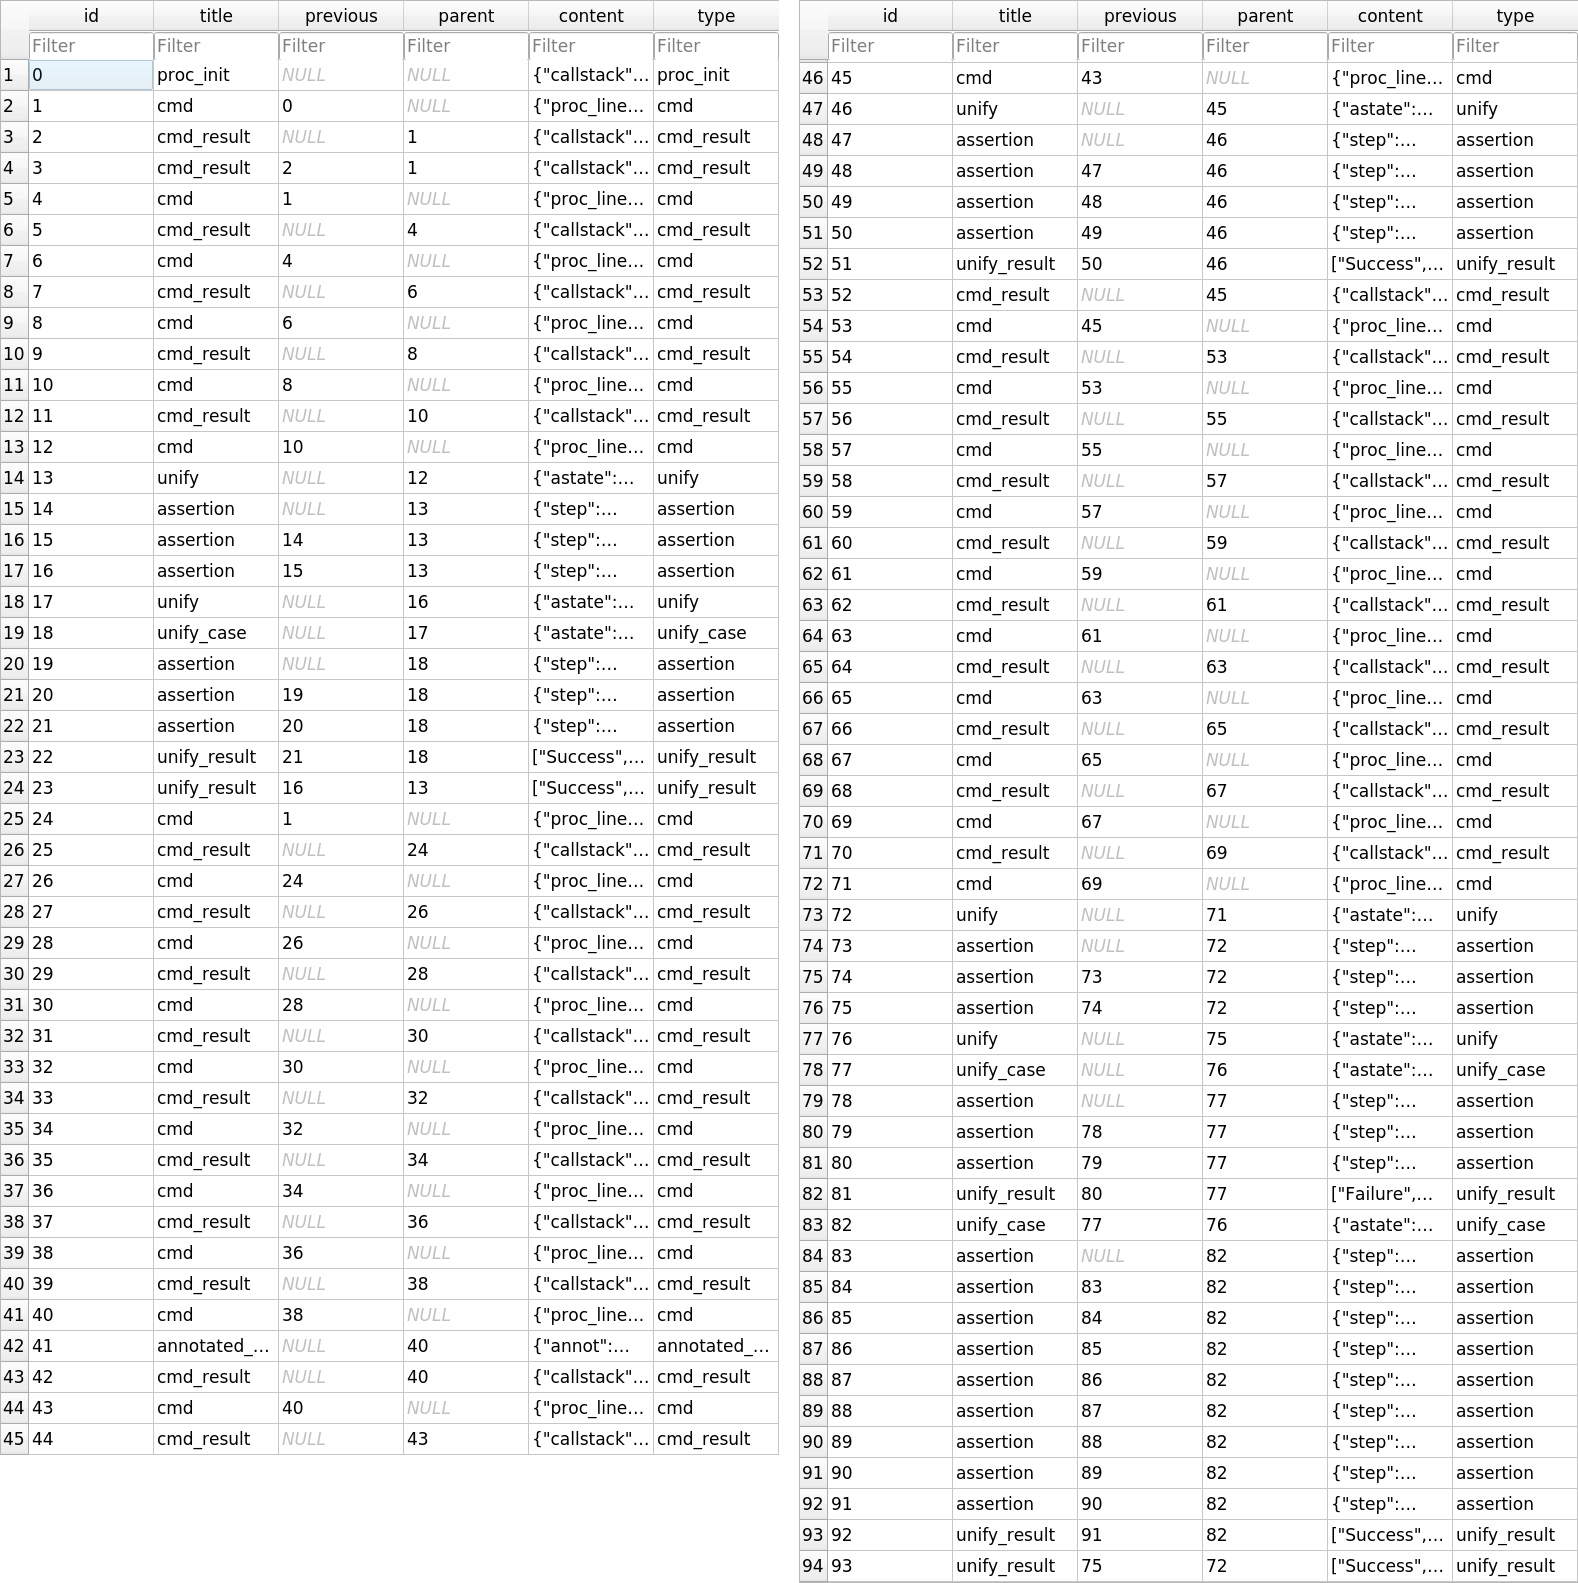
\includegraphics[width=0.8\textwidth]{img/log-structure-database.png}
  \caption{
    Evidence of the log structure being formed successfully in the database}%
  \label{fig:log-structure-database}
\end{figure}
